\documentclass[tikz,border=2mm]{standalone}

\tikzset{every picture/.append style={scale=1}}

\begin{document}

% 6 in the center + 1 and 2 in different positions

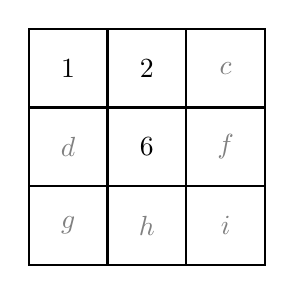
\begin{tikzpicture}
  \draw[line cap=rect, thick] grid(3, 3);
  \node at(0+0.5,2+0.5){$1$};
  \node at(1+0.5,2+0.5){$2$};
  \node at(2+0.5,2+0.5){\textcolor{gray}{$c$}};
  \node at(0+0.5,1+0.5){\textcolor{gray}{$d$}};
  \node at(1+0.5,1+0.5){$6$};
  \node at(2+0.5,1+0.5){\textcolor{gray}{$f$}};
  \node at(0+0.5,0+0.5){\textcolor{gray}{$g$}};
  \node at(1+0.5,0+0.5){\textcolor{gray}{$h$}};
  \node at(2+0.5,0+0.5){\textcolor{gray}{$i$}};
\end{tikzpicture}

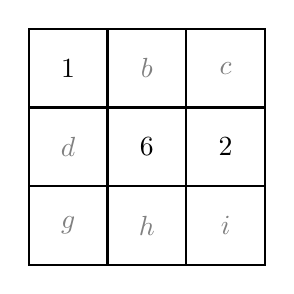
\begin{tikzpicture}
  \draw[line cap=rect, thick] grid(3, 3);
  \node at(0+0.5,2+0.5){$1$};
  \node at(1+0.5,2+0.5){\textcolor{gray}{$b$}};
  \node at(2+0.5,2+0.5){\textcolor{gray}{$c$}};
  \node at(0+0.5,1+0.5){\textcolor{gray}{$d$}};
  \node at(1+0.5,1+0.5){$6$};
  \node at(2+0.5,1+0.5){$2$};
  \node at(0+0.5,0+0.5){\textcolor{gray}{$g$}};
  \node at(1+0.5,0+0.5){\textcolor{gray}{$h$}};
  \node at(2+0.5,0+0.5){\textcolor{gray}{$i$}};
\end{tikzpicture}

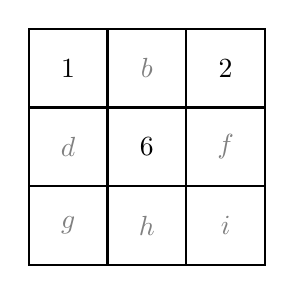
\begin{tikzpicture}
  \draw[line cap=rect, thick] grid(3, 3);
  \node at(0+0.5,2+0.5){$1$};
  \node at(1+0.5,2+0.5){\textcolor{gray}{$b$}};
  \node at(2+0.5,2+0.5){$2$};
  \node at(0+0.5,1+0.5){\textcolor{gray}{$d$}};
  \node at(1+0.5,1+0.5){$6$};
  \node at(2+0.5,1+0.5){\textcolor{gray}{$f$}};
  \node at(0+0.5,0+0.5){\textcolor{gray}{$g$}};
  \node at(1+0.5,0+0.5){\textcolor{gray}{$h$}};
  \node at(2+0.5,0+0.5){\textcolor{gray}{$i$}};
\end{tikzpicture}

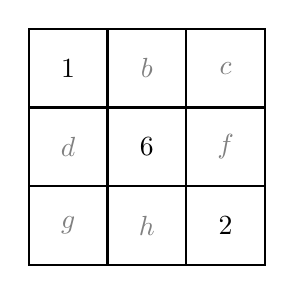
\begin{tikzpicture}
  \draw[line cap=rect, thick] grid(3, 3);
  \node at(0+0.5,2+0.5){$1$};
  \node at(1+0.5,2+0.5){\textcolor{gray}{$b$}};
  \node at(2+0.5,2+0.5){\textcolor{gray}{$c$}};
  \node at(0+0.5,1+0.5){\textcolor{gray}{$d$}};
  \node at(1+0.5,1+0.5){$6$};
  \node at(2+0.5,1+0.5){\textcolor{gray}{$f$}};
  \node at(0+0.5,0+0.5){\textcolor{gray}{$g$}};
  \node at(1+0.5,0+0.5){\textcolor{gray}{$h$}};
  \node at(2+0.5,0+0.5){$2$};
\end{tikzpicture}

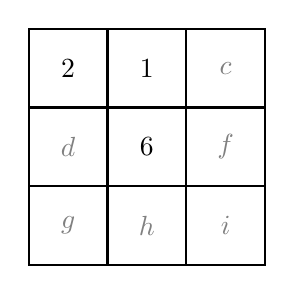
\begin{tikzpicture}
  \draw[line cap=rect, thick] grid(3, 3);
  \node at(0+0.5,2+0.5){$2$};
  \node at(1+0.5,2+0.5){$1$};
  \node at(2+0.5,2+0.5){\textcolor{gray}{$c$}};
  \node at(0+0.5,1+0.5){\textcolor{gray}{$d$}};
  \node at(1+0.5,1+0.5){$6$};
  \node at(2+0.5,1+0.5){\textcolor{gray}{$f$}};
  \node at(0+0.5,0+0.5){\textcolor{gray}{$g$}};
  \node at(1+0.5,0+0.5){\textcolor{gray}{$h$}};
  \node at(2+0.5,0+0.5){\textcolor{gray}{$i$}};
\end{tikzpicture}

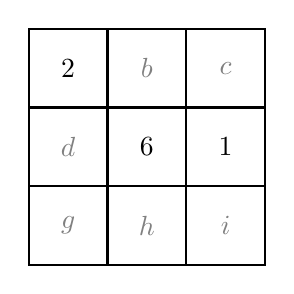
\begin{tikzpicture}
  \draw[line cap=rect, thick] grid(3, 3);
  \node at(0+0.5,2+0.5){$2$};
  \node at(1+0.5,2+0.5){\textcolor{gray}{$b$}};
  \node at(2+0.5,2+0.5){\textcolor{gray}{$c$}};
  \node at(0+0.5,1+0.5){\textcolor{gray}{$d$}};
  \node at(1+0.5,1+0.5){$6$};
  \node at(2+0.5,1+0.5){$1$};
  \node at(0+0.5,0+0.5){\textcolor{gray}{$g$}};
  \node at(1+0.5,0+0.5){\textcolor{gray}{$h$}};
  \node at(2+0.5,0+0.5){\textcolor{gray}{$i$}};
\end{tikzpicture}

% candidate that ends up being ruled out
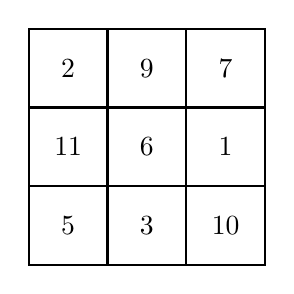
\begin{tikzpicture}
  \draw[line cap=rect, thick] grid(3, 3);
  \node at(1+0.5,1+0.5){$6$};
  \node at(2+0.5,1+0.5){$1$};
  \node at(0+0.5,2+0.5){$2$};
  \node at(1+0.5,0+0.5){$3$};
  \node at(0+0.5,0+0.5){$5$};
  \node at(2+0.5,2+0.5){$7$};
  \node at(1+0.5,2+0.5){$9$};
  \node at(2+0.5,0+0.5){$10$};
  \node at(0+0.5,1+0.5){$11$};
\end{tikzpicture}

\end{document}
